%% ****** Start of file apsguide4-1.tex ****** %
%%
%%   This file is part of the APS files in the REVTeX 4.1 distribution.
%%   Version 4.1r of REVTeX, August 2010.
%%
%%   Copyright (c) 2009, 2010 The American Physical Society.
%%
%%   See the REVTeX 4.1 README file for restrictions and more information.
%%
\documentclass[twocolumn,secnumarabic,amssymb, nobibnotes, aps, prd]{revtex4-1}
%\usepackage{acrofont}%NOTE: Comment out this line for the release version!
\newcommand{\revtex}{REV\TeX\ }
\newcommand{\classoption}[1]{\texttt{#1}}
\newcommand{\macro}[1]{\texttt{\textbackslash#1}}
\newcommand{\m}[1]{\macro{#1}}
\newcommand{\env}[1]{\texttt{#1}}
\setlength{\textheight}{9.5in}



\usepackage{color}
\usepackage[latin9]{inputenc}
\usepackage{mathrsfs,amsmath}
\usepackage{graphicx}%
\usepackage{float}
\usepackage{amsfonts}%
\usepackage[titletoc]{appendix}
\usepackage{amssymb}
\usepackage{braket}
\usepackage{bm}

\newcommand{\mb}[1]{\bm{#1}}
\usepackage[T1]{fontenc}

\def\Nabla{\bm{\nabla}}
\def\bm{\mathbf}
\def\curl{\Nabla\times}
\def\div{\Nabla\cdot}
\def\lap{\Delta}
\def\vlap{\Delta}
\def\x{\hat{e}_{x}}
\def\y{\hat{e}_{y}}
\def\z{\hat{e}_{z}}
\def\p{\partial}
\def\h{\hat}
\DeclareMathOperator{\Tr}{Tr}


\begin{document}

\title{Slow Terahertz Light via Resonant-tunneling Induced Transparency in Quantum Well Heterostructures}%

\author{Petar Tzenov}%
\email{petar.tzenov@tum.de}
\affiliation{Institute for Nanoelectronics, Technical University of Munich, D-80333 Munich, Germany}
\date{June 6, 2016}%
\maketitle
\tableofcontents

\section{Introduction}
We will theoretically and numerically demonstrate the possibility of achieving slow light in artificially designed atoms based on quantum well heterostructures.

Let us consider a simple toy configuration, consisting of two quantum wells, which we will refer to as the left and right well according to their relative positions, separated by a thick tunneling barrier. Let us assume that 
at design bias, the tight-binding basis ground state, $\Ket{s}$, of the left well aligns with  the first excited state $\Ket{e}$ of the right well, with some small detuning energy $E_{s}-E_{e} = \hbar \epsilon$. On the other hand, let us assume that the energetic difference between the state $\Ket{e}$ and the ground state of the right well, $\Ket{g}$ is given as $E_{e}- E_{g} = \hbar\omega_0 $, which can be assumed to lie in the terahertz (THz) range. 

In the tight binding basis, the alignment between the left ground state and the right excited state causes an energetic splitting, characterized by the anticrossing energy $\hbar\Omega_{se}$. Finally assuming an incident terahertz electromagnetic field $E(x,t)$, oscillating with central frequency $\omega_c$, which is near resonance with the $\Ket{e}\leftrightarrow\Ket{g}$ transition, i.e. $\omega_0 \approx \omega_c$, we can write down the tight-binding Hamiltonian of the system within the electric dipole approximation as

\begin{align}
	\label{eq:hamiltonian-operatorform}
	\h{H} &= \hbar(\epsilon + \omega_0) \h\sigma_{s,s} +\hbar\omega_0\h\sigma_{e,e}  \nonumber \\ 
	& +(\hbar\Omega_{se}\h\sigma_{s,e} +q_0d_{eg}E\h\sigma_{e,g}+h.c.),
\end{align}
where we have set the zero energy as the ground state energy, $d_{eg}=\Bra{e}\h z \Ket{g}$  denotes the dipole moment matrix element, $\h z$ is the position operator along the growth direction $z$, $q_0$ is the elementary charge and finally $\h \sigma_{i,j}$ are the atomic projection operators. Taking the states $\Ket{s},\Ket{e}$ and $\Ket{g}$ as a complete orthonormal basis,  the Hamiltonian in Eq. (\ref{eq:hamiltonian-operatorform}) can be cast into matrix form as

\begin{align}
\label{eq:hamiltonian-matrixform}
H &= \begin{pmatrix}
\hbar(\epsilon + \omega_0) & \hbar \Omega_{se} & 0 \\ 
\hbar \Omega_{se} & \hbar\omega_0 & q_0d_{eg}E \\
0 & q_0d_{eg}E & 0
\end{pmatrix}.
\end{align}

To model the light-matter interaction dynamics we will employ a density matrix approach to describe the statistical behaviour of the atomic ensemble in our system, coupled to the classical Maxwell's equations via a polarization term. 

Having assumed that the set $B:= \{\Ket{s},\Ket{e}$,$\Ket{g}\}$ is complete, we can write any arbitrary state $\Ket{\Psi_k}, k = 1,2,3$ of the electron as a coherent superposition of those basis levels, i.e. 
\begin{equation}
\Ket{\Psi_k} = \alpha_s^k \Ket{s} + \alpha_{e}^k\Ket{e} + \alpha_g^k\Ket{g}, 
\end{equation}
where $\alpha_j^k = \braket{j|\Psi_k}, \Ket{j} \in B$ and necessarily $|\alpha_s^k|^2+|\alpha_e^k|^2+|\alpha_g^k|^2 = 1$ (normalization condition). 

Assuming that $p_k$ is the classical probability of the system to be in state $\ket{\Psi_k}$, the density matrix of this ensemble can be written as:
\begin{align}
\label{eq:densitymatrix-operator}
\h \rho = \sum_{k=1}^3 p_k \ket{\Psi_k}\bra{\Psi_k} = \sum_{k=1}^3 p_k \sum_{i,j \in B}(\alpha_j^k)^*\alpha_i^k\ket{i}\bra{j}, 
\end{align}
where $^*$ denotes the complex conjugate. In the $B$ basis the density matrix elements $\rho_{i,j} = \braket{i|\h \rho| j}$ can be written as
\begin{equation}
\label{eq:dmelements}
\rho_{i,j} = \sum_{k=1}^{3} p_k \alpha_i^k(\alpha_j^k)^*.
\end{equation}
The physical interpretation of $\rho_{i,i} = \sum_{k=1}^{3} p_k |\alpha_i^k|^2 > 0 $ is straightforward, i.e. it is the weighted sum for the quantum mechanical probability of each ket $\Ket{\Psi_k}$ to be in basis state $\ket{i}$, with weights being the ensemble's probability to be in coherent state $\Psi_k$, i.e. the above expression incorporates both classical and quantum mechanical averaging, with the former inherent from our lack of knowledge about the system, and the latter from the purely QM nature of things. The off-diagonal terms of the density matrix, $\rho_{i,j}$ when $i\neq j$, do not have such an easy interpretation. They are usually called coherences and intuitively reflect the coupling strength between basis levels $\ket{i}$ and $\ket{j}$ in the statistical mixture. Lastly, the density matrix satisfies the normalization condition $\sum_i \rho_{i,i} = 1$, i.e.  $( \Tr{\rho} = 1)$. 

The time evolution of the density matrix is governed by the von Neumann equation
\begin{equation}
\frac{d \rho}{dt} = \frac{i}{\hbar} [\rho,H],
\end{equation}
where $[\cdot,\cdot]$ is the matrix commutator. Additionally there need to be included phenomenological scattering terms to model non-radiative incoherent scattering processes between different subbands of our system. The final form of the equation of motion, which we will consider, is therefore
\begin{equation}
\frac{d \rho}{dt} = \frac{i}{\hbar} [\rho,H] + coll,  
\end{equation}
where $coll$ denotes all collision terms (include in detail later). Including space dependence and employing the slowly varying envelope and rotating wave approximation we get the following system of equations
\begin{center}
\begin{widetext}
\begin{subequations}
	\label{eq:threelevelmodel}
	\begin{align}
	 \frac{n}{c}\partial_t f &+ \partial_{x}f= -i\frac{N \Gamma q_0d_{eg} k_c}{\epsilon_0 n^2} \eta_{eg} - \frac{l_0}{2} f \label{eq:rtwave} \\
		\frac{d \rho_{ss}}{d t} 	&= i\Omega_{se} (\rho_{se} - \rho_{es})+ \Gamma_{es}\rho_{ee} + \Gamma_{gs}\rho_{gg}  -\Gamma_s\rho_{ss} \\
		\frac{d \rho_{ee}}{d t}	& = i\Omega_{se} (\rho_{es} - \rho_{se}) + i\frac{q_0d_{eg}}{2\hbar} \big (f^*\eta_{eg}- c.c. \big ) 
		 +\Gamma_{se}\rho_{ss} + \Gamma_{ge}\rho_{gg} - \Gamma_e \rho_{ee},  \\
		\frac{d \rho_{gg}}{d t}  &= -i\frac{q_0d_{eg}}{2\hbar} \big (f^*\eta_{eg} - c.c. \big )  + \Gamma_{sg}\rho_{ss}  +  \Gamma_{eg}\rho_{ee} - \Gamma_{gg}\rho_{gg} , \\
		\frac{d \rho_{se}}{d t}  &= -i\epsilon\rho_{se} +i \Omega_{se}(\rho_{ss} - \rho_{ee}) +i\frac{q_0d_{eg}}{2 \hbar}f^*\eta_{sg}- \Gamma_{\parallel se} \rho_{se},  \\
		\frac{d \eta_{eg}}{d t}   &= i(\omega_c - \omega_0)\eta_{eg} + i \frac{q_0d_{eg}}{2\hbar}f(\rho_{ee}-\rho_{gg})  - i\Omega_{se}\eta_{sg} - \Gamma_{\parallel eg}\eta_{eg}, \\
		\frac{d \eta_{sg}}{d t} &= i(\omega_c - \omega_0-\epsilon)\eta_{sg} +i \frac{q_0d_{eg}}{2\hbar}f\rho_{se} - i\Omega_{se}\eta_{eg} - \Gamma_{\parallel sg}\eta_{sg}.
	\end{align}
\end{subequations}
\end{widetext}
\end{center}
We have made the following assumptions
\begin{align}
E(x,t) &= \frac{1}{2} (f(x,t) e^{i(k_cx-\omega_c t)}+c.c.),\\
\rho_{eg} &= \eta_{eg}e^{i(k_cx-\omega_c t)}, \\
\rho_{sg} &= \eta_{sg}e^{i(k_cx-\omega_c t)}, 
\end{align}
and $\Gamma_{ij} $ are the scattering rates from state $\ket{i}$ to state $\ket{j}$, $\Gamma_k = \sum_{j}\Gamma_{kj}$ is the total out-scattering rate from level $\ket{k}$ and $\Gamma_{\parallel ij} = \frac{1}{2}(\Gamma_{i} + \Gamma_j) + \Gamma_{i,j}^*$ with $\Gamma_{i,j}^*$ the pure dephasing rate for the transition $i\rightarrow j$. 

The linear polarization is given by
\begin{align}
P(x,t) &=\epsilon_0 \chi^{(1)} E(x,t) = \epsilon_0 \chi^{(1)} \frac{1}{2}( f(x,t) e^{i(k_cx-\omega_c t)}+c.c.) \nonumber \\  
	  &= -N\Gamma q_0d_{eg}(\eta_{eg}(x,t)e^{i(k_cx-\omega_c t)} + c.c.),
\end{align}
from where it follows that the linear susceptibility $\chi^{(1)}$ can be expressed as
\begin{align}
\chi^{(1)} &= -2\frac{N\Gamma q_0d_{eg}}{\epsilon_0 } \eta_{eg}(x,t)/f(x,t).
\end{align}
The steady state solution of $\eta_{eg}$ is directly computed from Eq. (\ref{eq:threelevelmodel}) and in the weak field limit (i.e. $|q_0d_{eg}f/\hbar| << |\Omega_{se}|$) we get the following expression
\begin{align}
\eta_{eg}  &= -[ \frac{\Omega_{se}^2}{ \gamma_{se} \big[\gamma_{sg}\gamma_{eg} -\Omega_{se}^2\big ] }\times (\rho_{ss}-\rho_{ee})  \nonumber \\
		 &+ \frac{\gamma_{sg}}{\big[\gamma_{sg}\gamma_{eg} -\Omega_{se}^2\big ] }\times (\rho_{ee}-\rho_{gg}) ]\times \frac{q_0d_{eg}}{\hbar}f(x,t). 
\end{align}
where we have defined $\gamma_{sg} =(\delta\omega - \epsilon + i\Gamma_{\parallel sg}) $, $\gamma_{eg} =(\delta\omega + i\Gamma_{\parallel eg})$, $\gamma_{se} = \epsilon - i\Gamma_{\parallel se}$ and $\delta\omega = \omega_c-\omega_0$ is the detuning of the probe field from resonance. In the strong tunneling coupling regime, the populations of $\ket{s}$ and $\ket{e}$ are almost equal therefore the linear susceptibility simplifies to
\begin{align}
\chi^{(1)} &= 2\frac{N\Gamma q_0^2d_{eg}^2}{\epsilon_0 \hbar}  \times \frac{\gamma_{sg}}{\gamma_{sg}\gamma_{eg} -\Omega_{se}^2  }\times (\rho_{ee}-\rho_{gg}),
\end{align}
which is the standard expression for the linear susceptibility of the 3 level $\Lambda$-system, known from the theory of electromagnetically induced transparency. 

Let us also assume a background susceptibility $\chi_0 = n^2-1$, assumed to be constant for narrow frequencies around the central carrier frequency. Then the total (complex) refractive index $\underline{n}$ is given by
\begin{equation}
\underline{n}^2 = n^2+\chi^{(1)},   
\end{equation}
where we have used the relation $ \underline{n}^2 = \chi_{tot} -1 = \chi_{0} + \chi^{(1)} - 1 = n^2 + \chi^{(1)}$. Taylor expanding around zero we finally obtain the complex refractive index as
\begin{equation}
	\underline{n} = n+\frac{1}{2n}\chi^{(1)}= n(1+r\Omega_p\times \frac{\gamma_{sg}}{\gamma_{sg}\gamma_{eg} -\Omega_{se}^2  }),
\end{equation}
where $r = \rho_{ee} - \rho_{gg}$ is the population inversion factor, and $\Omega_p = N\Gamma q_0^2d_{eg}^2/n^2\epsilon_0\hbar > 0$ is the modified plasma frequency. Assuming $\epsilon \approx 0$, the group refractive index is then given by 
\begin{align}
\label{eq:ngroup}
	n_g &= n +\omega_c  \left .\Re\{\frac{\p \underline{n}}{\p \delta\omega} \}\right |_{\delta \omega = 0} \nonumber \\
		&= n\Big (1-r\omega_c\Omega_p \times \frac{\Omega_{se}^2 -\Gamma_{\parallel sg}^2} {[\Omega_{se}^2 +\Gamma_{\parallel sg}\Gamma_{\parallel eg}]^2}  \Big).
\end{align}

From Eq. (\ref{eq:ngroup}), whenever the levels $\ket{s}$ and $\ket{g}$ have a very long coherence time, we can extract the necessary conditions for slow/superluminal light near the transparency window as follows:
\begin{enumerate}
	\item Slow light - achieving slow light requires very large positive group refractive index. Due to the positivity of $\Omega_p$ it therefore follows that we need our system to satisfy $r=\rho_{ee}-\rho_{gg} <0 $, i.e. un-inverted medium, and also $ |r| \Omega_p >> \Omega_{se}^2/\omega_c$. 
	\item Superluminal light - on the other hand it is also theoretically possible to achieve refractive indices $0<n_g<1$. It can be easily seen that the superluminal light condition cannot be fulfilled for un-inverted medium, i.e. 
	for $r < 0$, however one can achieve group velocities higher than $c$ if the following relation is satisfied
	\begin{equation}
	\label{eq:superluminal}
		\frac{n-1}{n}\frac{\Omega_{se}^2}{\omega_c} < r\Omega_p < \frac{\Omega_{se}^2}{\omega_c}, 
	\end{equation}   
	in an inverted medium, i.e. for $r > 0$.
\end{enumerate}

Typical values for the above parameters in the case of Quantum Well heterostructures can be summarized in the table below

	\begin{table}[H]
		\centering
		\footnotesize
		\begin{tabular}{ l | c c c }	
			\hline 
			{Refractive index }  & $n$ &   $\approx 3.6$ & (dimensionless) \\
			{Overlap factor}  & $\Gamma$ &   $\approx 0.95$ & (dimensionless) \\
			{Dipole moment}  & $d_{eg}$ &   $2 < d_{eg} < 5 $ & nm \\
			{Coupling energy}  & $\hbar \Omega_{sg}$ &  $0.5 <\hbar \Omega_{sg} < 1.5$ & meV \\
			{Trans. energy}  & $\hbar\omega_{0}$ & $9 <\hbar\omega_{0}< 12$ & meV \\
			{Carrier density}  & $N$ & $1\times10^{21} <N<  1\times10^{22}$ & $m^{-3}$\\
			\hline 
		\end{tabular}
		\caption[Table caption text]{ CAPTION TEXT}
		\label{tab:table02}
	\end{table}

Now in order to satisfy the slow light condition we choose the optimal values from the table above, in order to maximize the ratio $ |r| \Omega_p / \Omega_{se}^2/\omega_c$. Parameters susceptible to engineering are namely the dipole matrix element, which we set $ d_{eg} = 5$ nm, the anticrossing energy $\hbar\Omega_{sg} = 0.5 $ meV, the transition energy $\hbar \omega_0 = 12$ meV and the doping density $N = 1\times 10^{22} m^{-3}$. This gives us the ratio
$$
\frac{n_g}{n} = 1+|r|\Omega_p\times\frac{\omega_0}{\Omega_{se}^2} \approx  16.917
$$
or almost 17-fold slowdown of the group velocity with respect to the carrier frequency's phase velocity $c/n$. 

Next, let us investigate the effect of decoherence on the buffer performance. 
\subsection{Transparency under decoherence}
In case of strong $\ket{e}\leftrightarrow\ket{g}$ and $\ket{s}\leftrightarrow\ket{g}$ decoherence the transparency window will be significnatly reduced. To investigate this dependency we define the power transmittance over 
propagation length dL as
\begin{align}
T(\omega) = \exp(-2\omega c^{-1} \Im \{\underline{n}(\omega)\}dL)
\end{align}
The imaginary part of $\underline{n}(\omega)$ for $\epsilon = 0$ is given by
\begin{align}
n^{''}(\omega) = -nr\Omega_p\times \frac{\Gamma_{\parallel eg}(\Gamma_{\parallel sg}^2+\delta\omega^2) + \Omega_{se}^{2}\Gamma_{\parallel sg}}{(\delta\omega^2-\Gamma_{\parallel eg}\Gamma_{\parallel sg}-\Omega_{se}^2)^2+\delta\omega^2(\Gamma_{\parallel eg}+\Gamma_{\parallel sg})^2}.
\end{align}
Due to the exponential 


\section{Spectral hole burning due to strong injector anticrossing}
 
The introduction of the coupling energy $\hbar \Omega_{se}$ into the Hamiltonian of the system contributes to a splitting of the optical spectra into a high and a low frequency lobes. This is due to the fact that the extended system's Hamiltonian is non-diagonal in the tight binding basis. The new eigenstates, which diagonalize the Hamiltonian in Eq. (\ref{eq:hamiltonian-matrixform}), are the so called dressed states and are obtained from $\Ket{s}$ and $\Ket{e}$ via the unitary transformation
 \begin{align}
 \label{eq:dressedstates}
 \Ket{+} &= \cos\theta \Ket{s} - \sin\theta \Ket{e}, \nonumber \\
 \Ket{-} &= \sin\theta \Ket{s} + \cos\theta \Ket{e}.
 \end{align}
 The corresponding energies are given by $E_\pm =\hbar(\omega_0 +\frac{\epsilon}{2}) \pm \hbar\sqrt{\epsilon^2+4\Omega_{se}^2}$, where the coefficients are computed from  
 $
 \tan \theta = -2\Omega_{se}/(\epsilon+\sqrt{\epsilon^2+4\Omega_{se}^2}).
 $
 Here we remind the reader that the detuning from $\Ket {s}\leftrightarrow\Ket{e}$ resonance is given by $E_{s} - E_{e} = \hbar\epsilon$. We can compute the ratio of the dipole matrix elements for the $\Ket{+}\leftrightarrow\Ket{g}$ and $\Ket{-}\leftrightarrow\Ket{g}$ transitions, which will determine the relative strength between the high and low frequency lobes of the gain. Thus
 \begin{align}
 \label{eq:dresseddipoles}
 \left |\frac{\Bra{+}\hat{\mu}\Ket{g}}{\Bra{-}\hat{\mu}\Ket{g}}\right | \approx |\tan\theta| =  \frac{2|\Omega_{se}|}{|\epsilon+\sqrt{\epsilon^2+4\Omega_{se}^2}|},
 \end{align}
 where we assume that $\mu_{sg} \approx 0$.
 We now can easily see that at high biases, i.e. positive detunings $\epsilon >0$, $|\tan\theta|<1$ and thus the low frequency transition will have higher probability. On the other hand, for $\epsilon < 0 $ we get that $|\tan\theta| >1$ which will lead to lasing predominantly in the high frequency regime. This behaviour above and below resonant bias is schematically illustrated in Fig. \ref{fig:detuning}, where $\hbar\omega_{LF} $ and $\hbar\omega_{HF}$ denote the energy of the low and high frequency transition respectively and the anticrossing energy is set at $\hbar \Omega_{1'3} = 1$ meV.  
  \label{sec:biasdependence}
 \begin{figure}[h!]
 	\begin{center}
 		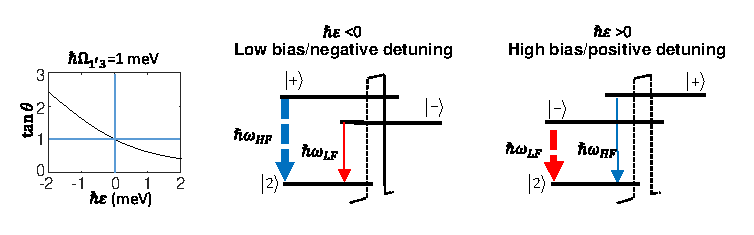
\includegraphics[scale=0.75]{BIASDETUNING.eps}
 		\caption{ Schematic illustration of the dependence of the high and low frequency transitions on bias. (Left column) Plot of $\tan\theta$ as a function of detuning from resonance. (Middle and right columns) The relative oscillator strengths (thicker arrow represents higher value) when the laser is biased below and above resonance, respectively. } \label{fig:detuning}
 	\end{center}	
 \end{figure}
\section{Temporal hole burning due to strong injector anticrossing}
Let us further investigate the effect of the spectral splitting onto the temporal dynamics of our system by taking the following, additional ansatz for the envelope $f(x,t)$ and accordingly the coherences
\begin{subequations}
	\begin{align}
	\label{eq:splittingAnsatz}
	f &= f^{(\delta)}e^{i(\delta k x  - \delta\omega t)} + f^{(-\delta)}e^{-i(\delta kx-\delta\omega t)}, \\
	\eta_{eg} &= \eta_{eg}^{(\delta)}e^{i(\delta k x  - \delta\omega t)} + \eta_{eg}^{(-\delta)}e^{-i(\delta kx-\delta\omega t)}, \\
	\eta_{sg} &= \eta_{sg}^{(\delta)}e^{i(\delta k x  - \delta\omega t)} + \eta_{sg}^{(-\delta)}e^{-i(\delta kx-\delta\omega t)},
	\end{align}
\end{subequations}
where $\delta\omega$ is \emph{half} the Rabi frequency of the tunneling transition. Next we use the above ansatz to evaluate the products $f^*\eta_{sg}$ and $f^*\eta_{eg}$ in Eq. (\ref{eq:threelevelmodel}) at $x=0$ (for convenience). Using the index $j$ as a place holder for $eg$ and  $sg$ we obtain
\begin{widetext}
	\begin{align}
	\label{eq:feta-product}
	f^{*}\eta_{j} &= ((f^{(\delta)})^*e^{  i\delta\omega t} + (f^{(-\delta)})^*e^{-i\delta\omega t})(\eta_{j}^{(\delta)}e^{ - i\delta\omega t} + \eta_{j}^{(-\delta)}e^{+i\delta\omega t}) \nonumber \\
	&= \big[ (f^{(\delta)})^*\eta_{j}^{(\delta)} +(f^{(-\delta)})^*\eta_{j}^{(-\delta)} + (f^{(\delta)})^*\eta_{j}^{(-\delta)}e^{2i\delta\omega t} + (f^{(-\delta)})^*\eta_{j}^{(\delta)}e^{-2i\delta\omega t}\big ].
	\end{align} 
\end{widetext}
We can reconciliate this result with Eq. (\ref{eq:threelevelmodel}) if we extend it with the following ansatz for the  population densities and the $\rho_{se}$ coherence term 
\begin{align}
\rho_{jj} &= \rho_{jj}^{DC}+\rho_{jj}^{+}e^{2i(\delta k x-\delta \omega t)} + \rho_{jj}^{-}e^{-2i(\delta k x-\delta \omega t)}, \\
\rho_{se} &= \rho_{se}^{DC}+\rho_{se}^{+}e^{2i(\delta k x-\delta \omega t)} + \rho_{se}^{-}e^{-2i(\delta k x-\delta \omega t)},
\end{align}
where $j \in \{s,e,g\}$, $\rho_{jj}^{-} = (\rho_{jj}^{(+)})^*$ and $\rho_{se}^{-} = (\rho_{es}^{+})^*$ due to the Hermitian property of the density matrix. Then, we can derive the evolution equations for $\rho_{jj}^{DC},\rho_{jj}^{\pm}$ and $\rho_{se}$ as follows (setting again x =0 for convenience)

\begin{widetext}
	\begin{align}
	\label{eq:temporal-hole-ss}
	\frac{d\rho_{ss}^{DC}}{dt} &= i\Omega_{se}(\rho_{se}^{DC}-\rho_{es}^{DC}) +  \Gamma_{es}\rho_{ee}^{DC} + \Gamma_{gs}\rho_{gg}^{DC}  -\Gamma_s\rho_{ss}^{DC}, \\
	\frac{d\rho_{ss}^{+}}{dt} &= 2i\delta\omega\rho_{ss}^{+} + i\Omega_{se}(\rho_{se}^{+}-\rho_{es}^{+}) +  \Gamma_{es}\rho_{ee}^{+} + \Gamma_{gs}\rho_{gg}^{+}  -\Gamma_s\rho_{ss}^{+}, \\
	\label{eq:temporal-hole-ee}
	\frac{d\rho_{ee}^{DC}}{dt} &= -i\Omega_{se}(\rho_{se}^{DC}-\rho_{es}^{DC}) + i\frac{q_0d_{eg}}{2\hbar} \left [ ( f^{(\delta)})^*\eta_{eg}^{(\delta)} +(f^{(-\delta)})^*\eta_{eg}^{(-\delta)} -c.c.\right]
	+\Gamma_{se}\rho_{ss}^{DC} + \Gamma_{ge}\rho_{gg}^{DC} - \Gamma_e \rho_{ee}^{DC}, \\
	\frac{d\rho_{ee}^{+}}{dt} &= 2i\delta\omega\rho_{ee}^{+} - i\Omega_{se}(\rho_{se}^{+}-\rho_{es}^{+}) + i\frac{q_0d_{eg}}{2\hbar} \left [ (f^{(-\delta)})^*\eta_{eg}^{(\delta)} -c.c.\right]
	+\Gamma_{se}\rho_{ss}^{+} + \Gamma_{ge}\rho_{gg}^{+} - \Gamma_e \rho_{ee}^{+}, \\
	\frac{d\rho_{gg}^{DC}}{dt} &= -i\frac{q_0d_{eg}}{2\hbar} \left [ ( f^{(\delta)})^*\eta_{eg}^{(\delta)} +(f^{(-\delta)})^*\eta_{eg}^{(-\delta)} -c.c.\right]
	+\Gamma_{sg}\rho_{ss}^{DC} + \Gamma_{eg}\rho_{ee}^{DC} - \Gamma_g \rho_{gg}^{DC}, \\
	\frac{d\rho_{gg}^{+}}{dt} &= 2i\delta\omega\rho_{gg}^{+} - i\frac{q_0d_{eg}}{2\hbar} \left [ (f^{(-\delta)})^*\eta_{eg}^{(\delta)} -c.c.\right]
	+\Gamma_{sg}\rho_{ss}^{+} + \Gamma_{eg}\rho_{ee}^{+} - \Gamma_g \rho_{gg}^{+}, \\
	\frac{d \rho_{se}^{DC}}{d t}  &= -i\epsilon\rho_{se}^{DC} +i \Omega_{se}(\rho_{ss}^{DC} - \rho_{ee}^{DC}) +i\frac{q_0d_{eg}}{2 \hbar}((f^{(\delta)})^*\eta_{sg}^{(\delta)} +(f^{(-\delta)})^*\eta_{sg}^{(-\delta)})- \Gamma_{\parallel se} \rho_{se}^{DC},  \\
	\frac{d \rho_{se}^{+}}{d t}  &= i(2\delta\omega-\epsilon)\rho_{se}^{+} +i \Omega_{se}(\rho_{ss}^{+} - \rho_{ee}^{+}) +i\frac{q_0d_{eg}}{2 \hbar}( (f^{(-\delta)})^*\eta_{sg}^{(\delta)} )- \Gamma_{\parallel se} \rho_{se}^{+},\\
	\frac{d \rho_{se}^{-}}{d t}  &= -i(2\delta\omega+\epsilon)\rho_{se}^{-} +i \Omega_{se}(\rho_{ss}^{-} - \rho_{ee}^{-}) +i\frac{q_0d_{eg}}{2 \hbar}( (f^{(\delta)})^*\eta_{sg}^{(-\delta)} )- \Gamma_{\parallel se} \rho_{se}^{-},  \\
	\frac{d \eta_{eg}^{(\pm\delta)}}{d t} &= i(\omega_c-\omega_0\pm \delta\omega)\eta_{eg}^{(\pm\delta)}
	+i\frac{q_0d_{eg}}{2\hbar} ( f^{(\pm\delta)}(\rho_{ee}-\rho_{gg})^{DC} + f^{(\mp \delta)} (\rho_{ee}-\rho_{gg})^{\pm})-i\Omega_{se}\eta_{sg}^{(\pm\delta)}- \Gamma_{\parallel eg}\eta_{eg}^{(\pm\delta)}, \label{eq:etase-temphole} \\
	\frac{d \eta_{sg}^{(\pm\delta)}}{d t} &= i(\omega_c-\omega_0-\epsilon \pm \delta\omega)\eta_{sg}^{(\pm\delta)}+i\frac{q_0d_{eg}}{2\hbar} ( f^{(\pm\delta)}\rho_{se}^{DC} + f^{(\mp \delta)} \rho_{se}^{\pm})-i\Omega_{se}\eta_{eg}^{(\pm\delta)}- \Gamma_{\parallel eg}\eta_{sg}^{(\pm\delta)}. \label{eq:etasg-temphole}
	\end{align} 
\end{widetext}

It is worthwhile to note that in the above derivation of Eq. (\ref{eq:etase-temphole},\ref{eq:etasg-temphole}) we have neglected terms proportional to $e^{\pm 3\delta \omega t}$. Finally, we can expand the wave propagation equations within our familiar ansatz and we see that the high and low frequency lobes satisfy
\begin{align}
\frac{n}{c}\partial_t f^{(\pm \delta)} + \partial_{x}f^{(\pm \delta)}&= -i\frac{N \Gamma q_0d_{eg} k_c}{\epsilon_0 n^2} \eta_{eg}^{(\pm \delta)} \nonumber \\ 
&- \left[\frac{l_0}{2}  \mp i (\frac{n\delta\omega}{c}-\delta k)\right] f^{(\pm \delta)}\label{eq:rtwave-temphole},
\end{align}
from where we see that in case of chromatic dispersion, i.e. the term is $(n\delta\omega/c-\delta k) \neq 0 $, is responsible for the difference in group velocities in the high and low lobe.

\end{document}

